%--------------------------------------------------------------------
\titreTD{\thenumTD}{Les structures de Lewis}
%--------------------------------------------------------------------

\begin{center}
\textit{Pour ce TD et le suivant, on se basera sur les ensembles ci-dessous~:}

\vrule

%\begin{tabular}{lllll}
%\hline
%\multicolumn{3}{l}{\textbf{Ensemble I}}\\
%\hline
%H$_2$O      & HCN      & PCl$_3$     & CH$_3^+$ & CH$_3^-$\\
%CH$_4$      & CH$_3$OH & C$_2$H$_6$~: CH$_3$CH$_3$ && \\
%NH$_3$      & HBr      & H$_2$S      &&\\
%NH$_2$OH    & SiH$_4$  & HCl         &&\\
%NF$_3$      & PH$_3$   & BH$_3$      &&\\
%\hline
%\end{tabular}
%
%\vspace{0.5cm}
%
%\begin{tabular}{lll}
%\hline
%\multicolumn{3}{l}{\textbf{Ensemble II}}\\
%\hline
%HC(CH$_3$)$_3$   & CH$_2$CHC(O)CH$_3$ & CH$_3$CH$_2$NH$_2$   \\
%H$_2$CO          & CH$_3$COOH         & CH$_3$C(O)NH$_2$     \\
%CH$_3$CHO        & HCOOH              & CH$_2$CHNHCH$_3$     \\
%CH$_3$CH$_2$CHO  & CF$_3$COOH         & C$_2$H$_2$           \\
%%CH$_2$CHCOH      & CH$_3$C(O)NH$_2$   & CH$_3$C(O)C(O)CH$_3$ \\
%\hline
%\end{tabular}
%\end{center}

\begin{tabular}{lll|lll}
\hline
\multicolumn{3}{c|}{\textbf{ENSEMBLE I}}            & \multicolumn{3}{c}{\textbf{ENSEMBLE II}}\\
\hline                                               
H$_2$O      & HCN      & PCl$_3$                   & HC(CH$_3$)$_3$   & CH$_2$CHC(O)CH$_3$ & CH$_3$CH$_2$NH$_2$   \\
CH$_4$      & CH$_3$OH & C$_2$H$_6$~: CH$_3$CH$_3$ & H$_2$CO          & CH$_3$COOH         & CH$_3$C(O)NH$_2$     \\
NH$_3$      & HBr      & H$_2$S                    & CH$_3$CHO        & HCOOH              & CH$_2$CHNHCH$_3$     \\
NH$_2$OH    & SiH$_4$  & HCl                       & CH$_3$CH$_2$CHO  & CF$_3$COOH         & C$_2$H$_2$           \\
NF$_3$      & PH$_3$   & BH$_3$                    & &&\\
CH$_3^+$    & CH$_3^-$ &                           & &&\\
\hline
\end{tabular}

\vrule
\end{center}

\exo{L'algorithme de Lewis}

Rappeler les \'etapes pour construire une structure de Lewis, exemple du CO$_2$ 
(C central).

%\subsubsection{Du squelette \`a la structure de Lewis}

%%

%%

\exo{Structure de Lewis de mol\'ecules simples}

Pour chaque atome des compos\'es de l'ensemble I (diff\'erents de H), indiquer sa position dans 
le tableau p\'eriodique (p\'eriode et groupe). Compter les \'electrons de valence,
envisager un squelette et donner 
la structure de Lewis de chaque compos\'e. \'Etablir la charge et le degr\'e
d'oxydation de chaque atome.

\exo{Structure de Lewis de mol\'ecules organiques simples}

Pour les mol\'ecules de l'ensemble II, \'etablir la structure de Lewis en suivant
l'exemple ci-dessous~:

%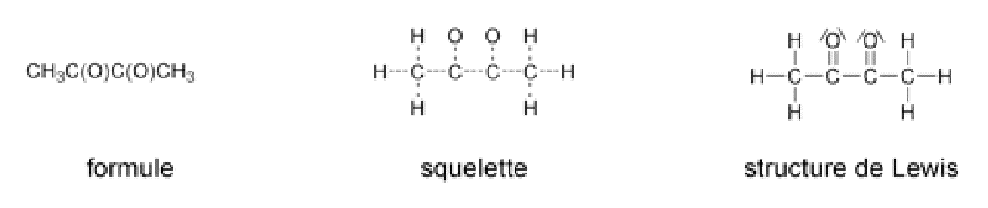
\includegraphics[width=13cm]{figure/Ex4_SLewis.eps}
%%
\begin{center}
\begin{tabular}{ccc}
\includegraphics[width=3cm]{figure/exlewis1.eps} &
\includegraphics[width=3cm]{figure/exlewis2.eps} &
\includegraphics[width=3cm]{figure/exlewis3.eps} \\
Formule & Squelette & Structure de Lewis \\
\end{tabular}
\end{center}

\exo{Degr\'e d'oxydation}

Pour les atomes de carbone en gras des structures suivantes, \'etablir le degr\'e
d'oxydation~:

\begin{center}
\begin{tabular}{lll}
CH$_3$\textbf{C}H$_2$OH     & CH$_3$CH$_2$\textbf{C}H$_2$OH & CH$_3$\textbf{C}H$_2$OCH$_3$ \\
CH$_3$\textbf{C}OOH         & CH$_3$\textbf{C}(O)OCH$_3$      & CH$_3$\textbf{C}HO           \\ 
CH$_3$CH$_2$\textbf{C}H$_3$ & CH$_3$\textbf{C}H$_2$CH$_3$   & CH$_3$\textbf{C}(O)NH$_2$      \\
HC\textbf{C}H               & HC\textbf{C}CH$_3$            & CH$_2$\textbf{C}HCH$_3$      \\ 
\end{tabular}
\end{center}

\exo{Structures de Lewis et p\'eriode 3}

Pour les syst\`emes suivants, \'etablir les structures de Lewis, la charge et le degr\'e
d'oxydation de chaque atome. Quel est la particularit\'e des \'el\'ements P, Cl et S dans ces compos\'es~?

{\small \textit{Pour construire le squelette de la mol\'ecule~: l'atome central est en gras et les atomes d'hydrog\`ene 
sont connect\'es aux atomes d'oxyg\`ene.}}

\vspace{0.5cm}

%\centerline{H$_3$\textbf{P}O$_4$, H$_3$\textbf{P}O$_2$, H$_2$\textbf{S}O$_4$, H\textbf{Cl}O, H\textbf{Cl}O$_4$.}
\centerline{H$_3$\textbf{P}O$_4$, H$_2$\textbf{S}O$_4$, H\textbf{Cl}O, H\textbf{Cl}O$_4$.}

\exo{Structures de Lewis \'equivalentes} 

Plusieurs structures de Lewis sont envisageables pour les mol\'ecules suivantes. 
Les \'etablir pour chaque mol\'ecule. 

\vspace{0.5cm}

\centerline{NO$_2^-$, HNO$_3$, SO$_4^{2-}$, SO$_3$, HCO$_3^-$, CO$_3^{2-}$, ClO$_4^-$, O$_3$.}

